\documentclass[12pt,a4paper]{article}

\usepackage[T2A]{fontenc}
\usepackage[utf8]{inputenc}
\usepackage[russian]{babel}

\usepackage{geometry}
\geometry{margin=2.5cm}

\usepackage{setspace}
\usepackage{indentfirst}
\usepackage{enumitem}
\usepackage{float}
\usepackage{booktabs}
\usepackage{array}
\usepackage{graphicx}
\usepackage{caption}

\setlength{\parskip}{0pt}
\setlength{\parindent}{1.25cm}

\begin{document}
\thispagestyle{empty}

\begin{center}
\textbf{МОСКОВСКИЙ АВИАЦИОННЫЙ ИНСТИТУТ}\\
\textbf{(НАЦИОНАЛЬНЫЙ ИССЛЕДОВАТЕЛЬСКИЙ УНИВЕРСИТЕТ)}
\end{center}

\vspace{2.2cm}

\begin{center}
\textbf{Институт №8 «Компьютерные науки и прикладная математика»}
\end{center}

\vspace{3.0cm}

\begin{center}
{\Large \textbf{Лабораторные работа}}\\[0.4cm]
{\Large \textbf{по курсу «Информационный поиск»}}
\end{center}

\vspace{4.0cm}

\begin{flushleft}
Выполнил: Гиголаев Антон Александрович\\
Группа: М8О-409Б-22\\
Преподаватель: Кухтичев Антон Алексеевич
\end{flushleft}

\vfill

\begin{center}
Москва, 2026
\end{center}

\newpage

\section*{1. Описание проекта}

Работа охватывает полный учебный конвейер информационного поиска: краулинг HTML-страниц, хранение в MongoDB, построение булевого инвертированного индекса и выполнение запросов из CLI и через WEB-интерфейс.

Корпус собран из Русской Википедии (ru.wikipedia.org) и Habr (habr.com). Все документы на русском языке; сохраняются сырые HTML и метаданные краулинга (URL, дата, хэш контента, источник).

\section*{2. Состав и структура репозитория}

Проект разбит на отдельные задачи:

\begin{itemize}[label=•, leftmargin=1.2em]
\item \texttt{task\_2} - краулер (C, libcurl + MongoDB C driver);
\item \texttt{task\_3} - токенизация и закон Ципфа (C + Python график);
\item \texttt{task\_4} - индексатор (C++ без STL, MongoDB input);
\item \texttt{task\_5} - поиск (CLI + WEB-интерфейс, C++ без STL);
\item \texttt{task\_6} - единый LaTeX отчёт.
\end{itemize}

Запуск и оркестрация выполняются через Docker Compose.

Ключевые сервисы Docker Compose:

\begin{itemize}[label=•, leftmargin=1.2em]
\item \texttt{mongo} - MongoDB 7 (порт 27017);
\item \texttt{crawler} - краулер;
\item \texttt{indexer} - построение индекса (профиль \texttt{tools});
\item \texttt{web} - веб-интерфейс поиска (порт 8080);
\item \texttt{cli} - CLI-поиск (профиль \texttt{tools}).
\end{itemize}

\section*{3. Корпус документов}

Корпус собирается краулером и хранится в MongoDB в базе \texttt{infosearch}. Сырые страницы записываются в коллекцию \texttt{pages}, после чего отдельная утилита извлекает текст и сохраняет его в \texttt{articles}. Для построения индекса используется именно \texttt{articles} (поля \texttt{url}, \texttt{text}, \texttt{title}, \texttt{author}, \texttt{published\_at}, \texttt{source}).

% AUTO:DOCS_BEGIN
Всего собрано документов: \textbf{19960}.
% AUTO:DOCS_END

\section*{4. Краулер}

Краулер написан на C и использует MongoDB для хранения результатов и состояния обхода. Реализованы:

\begin{itemize}[label=•, leftmargin=1.2em]
\item ограничение доменов (allow\_domains);
\item пауза между запросами, лимит глубины/страниц;
\item повторный обход и хранение хэша контента;
\item сохранение сырых HTML-страниц для последующей индексации.
\end{itemize}

В Docker-окружении используется подключение \texttt{mongodb://mongo:27017/}.

\section*{5. Индексация и токенизация}

Индексатор реализован на C++ без STL. На вход поступают документы из MongoDB, из HTML извлекается текст, затем выполняются токенизация и стемминг. После этого строится булев инвертированный индекс (термин → список документов).

Правила токенизации (как реализовано в коде):

\begin{itemize}[label=•, leftmargin=1.2em]
\item текст приводится к нижнему регистру;
\item токен - непрерывная последовательность букв/цифр (латиница и кириллица в UTF-8);
\item дефис и апостроф допускаются внутри токена, если окружены буквенно-цифровыми символами;
\item HTML-теги отбрасываются, управляющие символы игнорируются.
\end{itemize}

Стемминг: простой суффиксный отсекатель для русских слов (набор распространённых окончаний).

Замеры производительности индексатора (команда \texttt{ir\_indexer}, параметр \texttt{--limit}):

\begin{center}
\renewcommand{\arraystretch}{1.15}
\begin{tabular}{r r r r r r r}
\toprule
Docs & Terms & Tokens & Avg token len & Input, KB & Elapsed, s & Speed, KB/s\\
\midrule
% AUTO:TABLE_BEGIN
1000 & 19779 & 202545 & 8.92568 & 1412 & 0.25612 & 5513.8\\
5000 & 60829 & 1111798 & 8.96421 & 7793 & 1.00607 & 7746.5\\
10000 & 123792 & 4503575 & 9.54435 & 32132 & 3.89437 & 8250.8\\
19960 & 383124 & 20239398 & 9.67750 & 144089 & 20.81593 & 6922.1\\
% AUTO:TABLE_END
\bottomrule
\end{tabular}
\end{center}

\vspace{0.3cm}

Ниже приведены графики зависимости времени и скорости индексирования от объёма входных данных.

\begin{figure}[H]
  \centering
  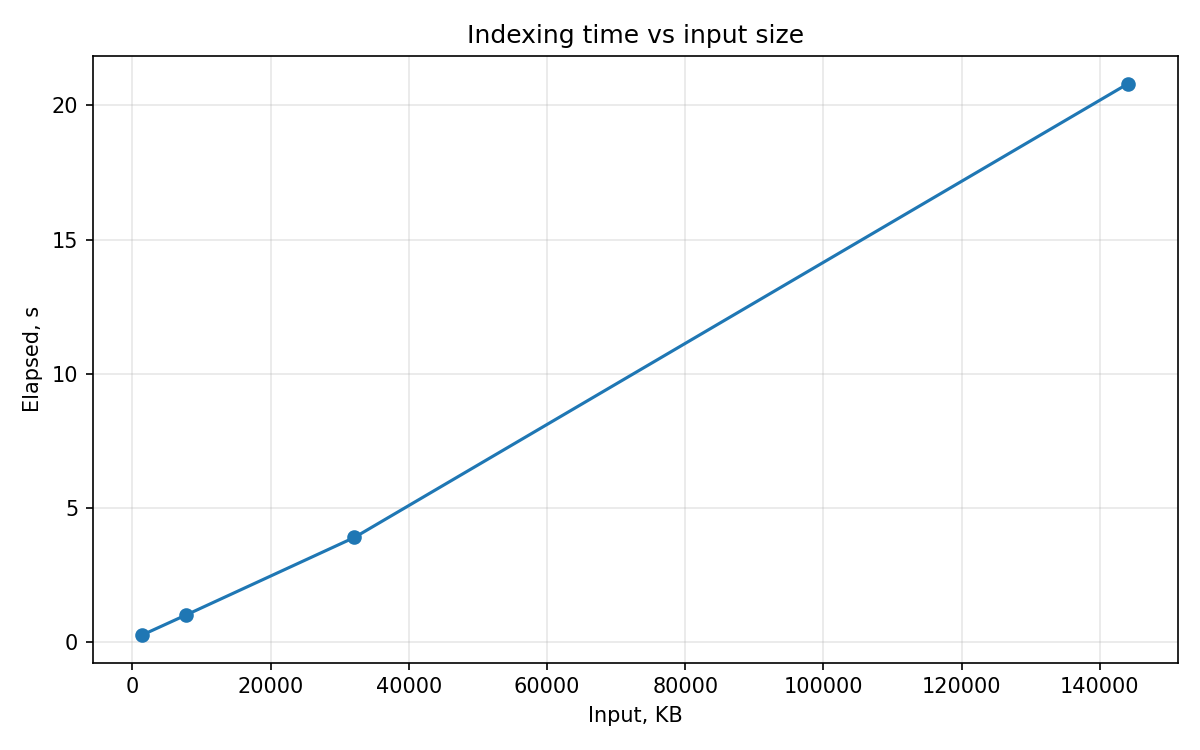
\includegraphics[width=\textwidth]{img/perf_time_vs_size.png}
\caption{Зависимость времени построения индекса от объёма входных данных.}
\end{figure}

\begin{figure}[H]
  \centering
  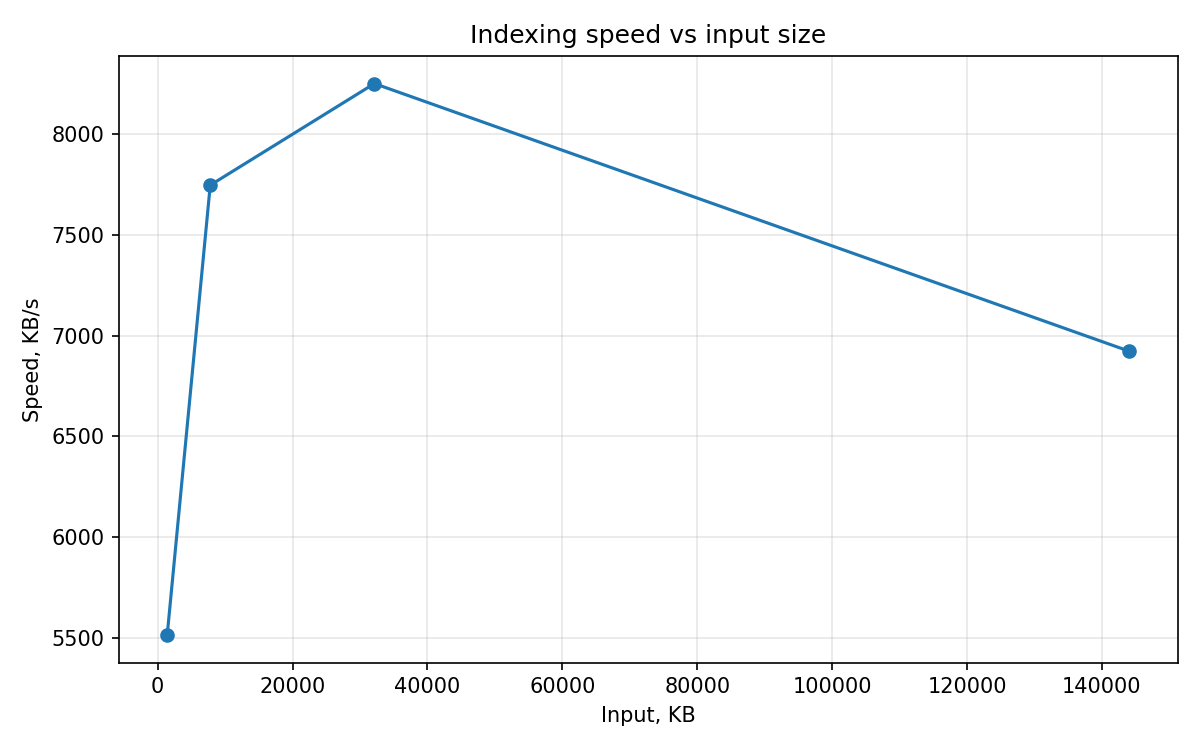
\includegraphics[width=\textwidth]{img/perf_speed.png}
\caption{Зависимость скорости токенизации+индексации от объёма входных данных.}
\end{figure}

\section*{6. Закон Ципфа}

Для корпуса построено распределение терминов по частотам в лог-лог шкале. На верхних рангах ожидаемо находятся служебные слова русского языка (и, в, на). Для повышения качества поиска такие слова можно исключать через стоп-лист.

\begin{figure}[H]
  \centering
  
\includegraphics[width=\textwidth]{img/zipf.png}
  \caption{Закон Ципфа и эмпирическое распределение терминов.}
\end{figure}

\section*{7. Булев поиск}

Поисковая подсистема поддерживает булевы операторы and, or, not и скобки. Запрос вычисляется над postings-списками: пересечение (AND), объединение (OR) и разность (NOT). Приоритет операторов: NOT > AND > OR; скобки задают порядок вычисления.

Реализованы два интерфейса:

\begin{itemize}[label=•, leftmargin=1.2em]
\item WEB-интерфейс на порту 8080 (форма поиска и HTML-выдача);
\item CLI-интерфейс.
\end{itemize}

\section*{8. Примеры работы WEB-интерфейса}

Ниже показаны примеры запросов и полученной выдачи.

\begin{figure}[H]
  \centering
  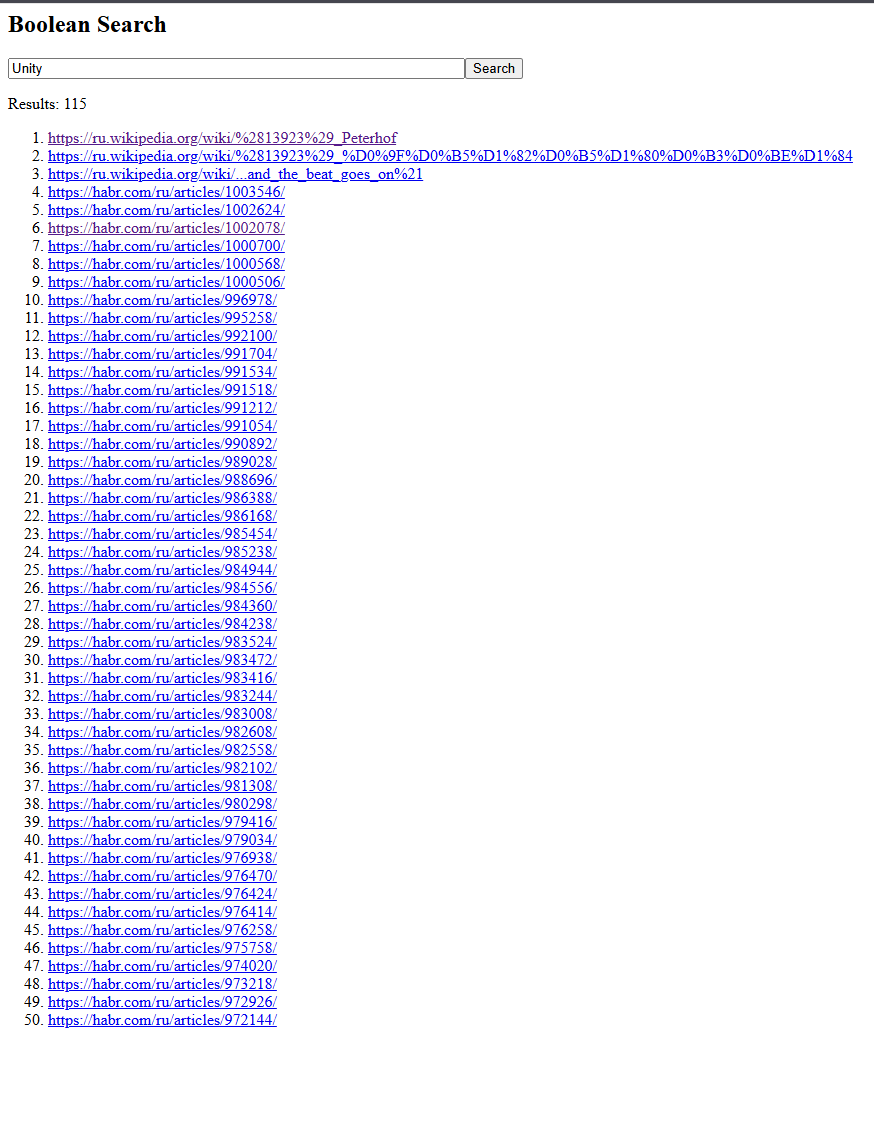
\includegraphics[width=\textwidth]{img/web_1.png}
\caption{Пример простого запроса: Unity}
\end{figure}

\begin{figure}[H]
  \centering
  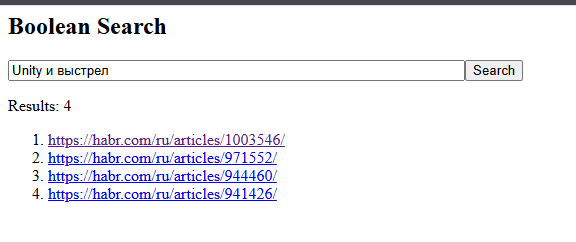
\includegraphics[width=\textwidth]{img/web_2.png}
\caption{Пример булевого запроса: Unity и выстрел.}
\end{figure}

\begin{figure}[H]
  \centering
  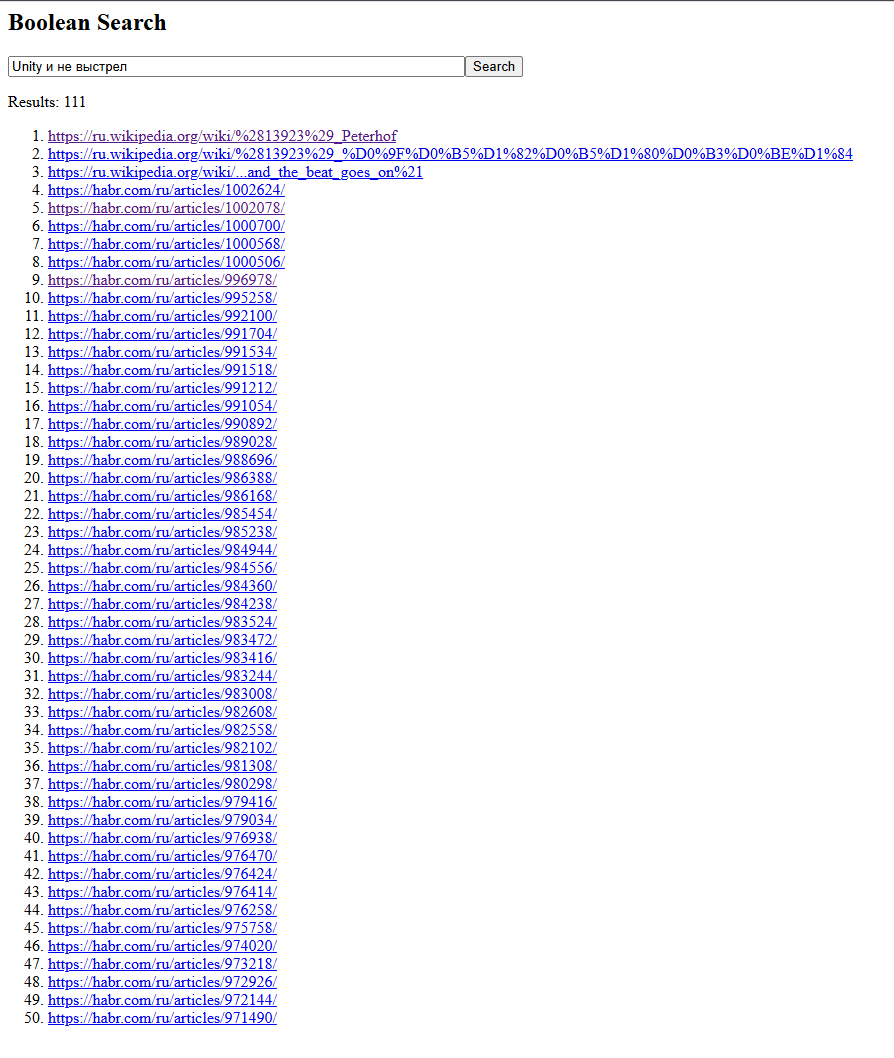
\includegraphics[width=\textwidth]{img/web_3.png}
\caption{Пример булевого запроса: Unity и не выстрел}
\end{figure}

\section*{9. Вывод}

Выполнен полный пайплайн информационного поиска: сбор корпуса (краулер), построение инвертированного булевого индекса и выполнение запросов через WEB и CLI. Проведены замеры производительности индексирования на разных объёмах входных данных, а также подготовлена статистика для анализа закона Ципфа.

\end{document}
